% 4
\section{アルゴリズム}
どのような流れで、プログラムが動作しているのか説明を行う。大まかな流れに分けると次のようになる。

\begin{enumerate}
 \item デバイスに設置した二台の'Webカメラから、それぞれ映像をキャプチャする。これらのカメラは縦、横に設置される。
 \item それぞれのキャプチャした画像上に、正方格子点が存在すると考える。点と重なる画素について、青色かどうか判定して結果を取得する。青色でない場合、何かしらの物体が存在すると判断する。
 \item 縦、横、それぞれの結果を組み合わせることで、3次元のデータを生成する。
 \item 三次元空間に、正方格子点が存在すると考える。この空間には、あらかじめデータを入力した三次元オブジェクトを配置している。すべての格子点について、このオブジェクトの内部にあるか外部にあるのかを判定して結果を取得する。
 \item 3で得た物体情報が格納された三次元データと、5で得た内部外部判定が格納された三次元データを比較する。3で物体が存在すると判断された点と、4で内部と判定された点が重なっている場合、物体はオブジェクトの内部に存在すると判断する。
 \item 物体がオブジェクト外部に出るように三次元オブジェクトを移動させる。
\end{enumerate}
 
本章では、2、3、4についてより詳細な説明を行う。

% 4.1
\subsection{カメラ画像からの物体データの取得}
縦に設置したWebカメラから得た画像について述べる。まず、Webカメラから取得した画像はRGB色空間での表現となっているため、特定の色が抽出しやすいHSV色空間への変換を行う。

 \vspace{5mm}
\begin{minipage}{0.5\hsize}
  \begin{center}
   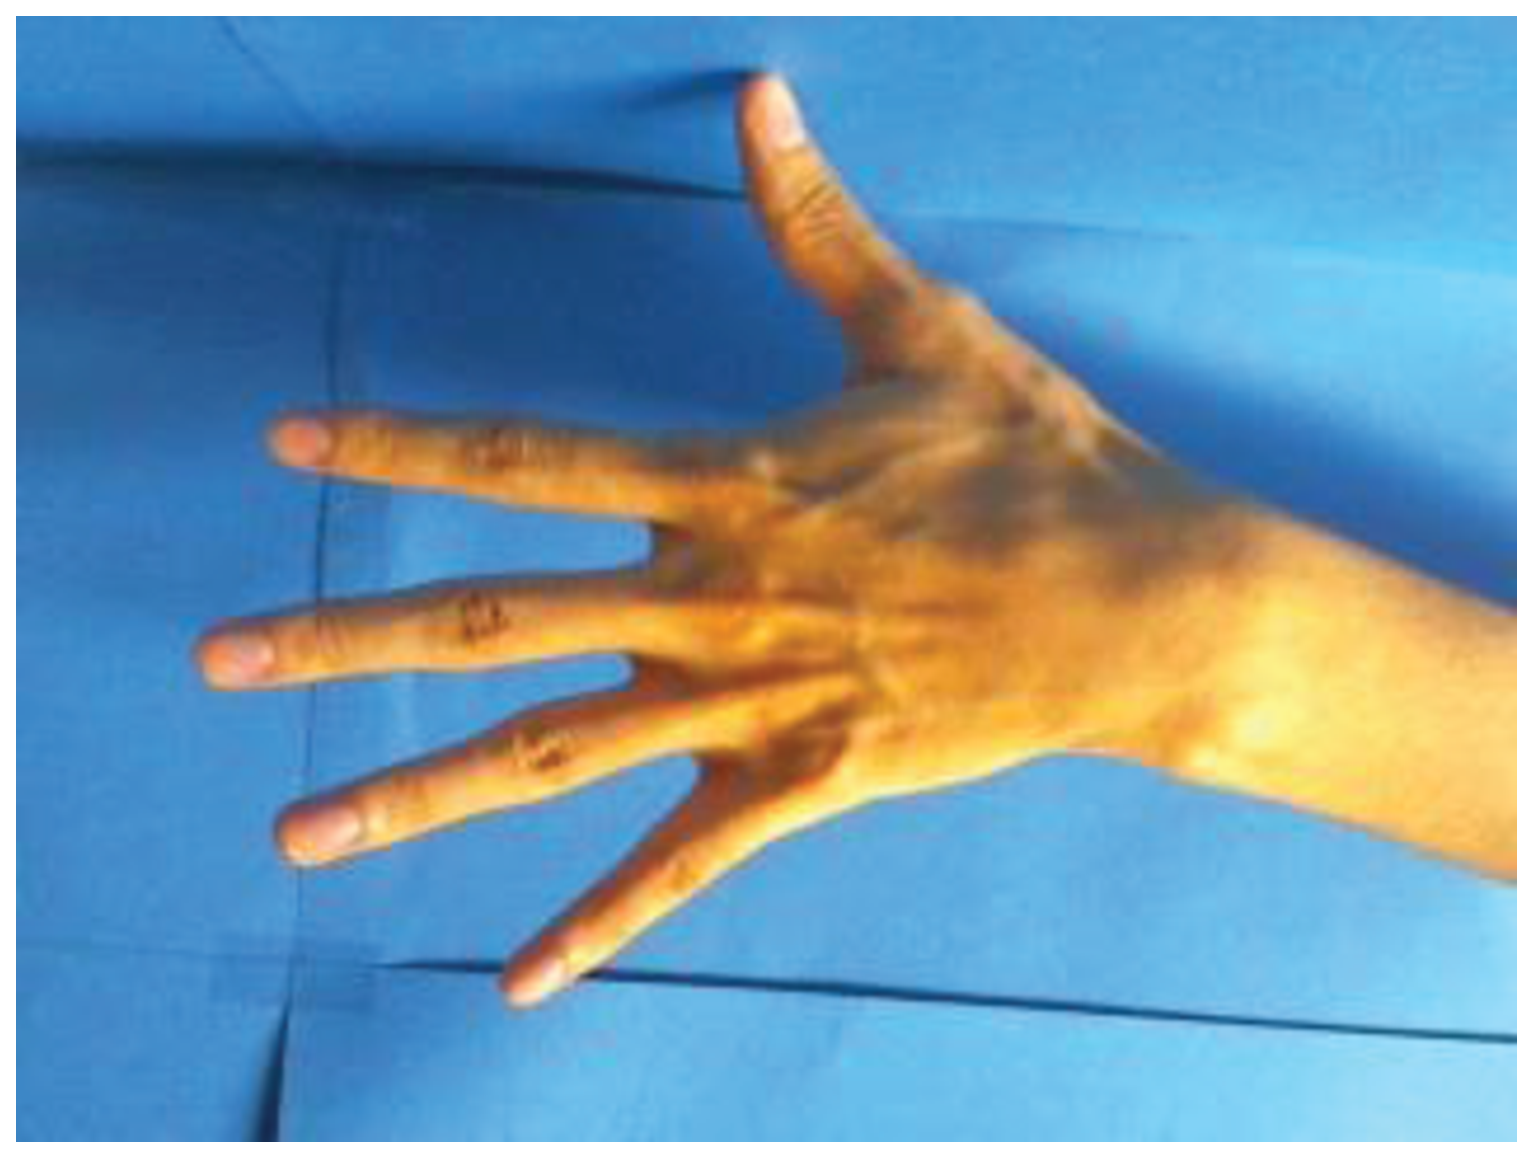
\includegraphics[width=70mm]{Simulator_getPic.eps}
   図4-1. RGB空間での表現
  \end{center}
  \label{fig:one}
 \end{minipage}
 \begin{minipage}{0.5\hsize}
  \begin{center}
   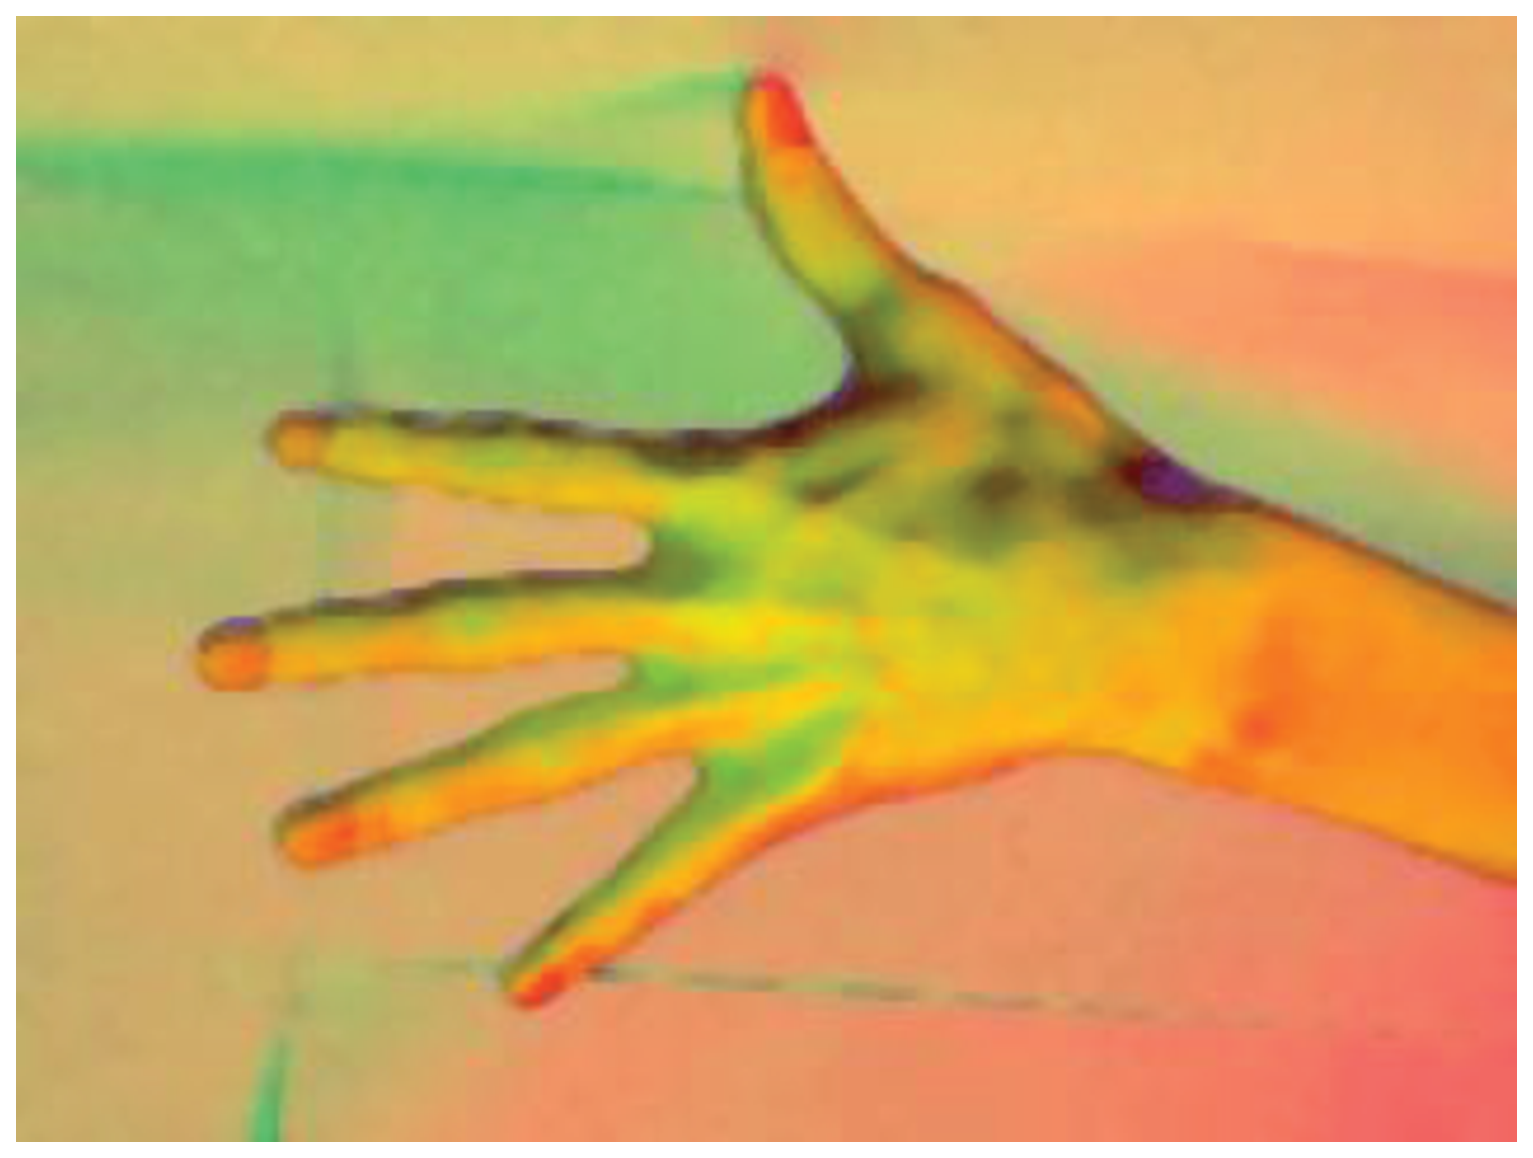
\includegraphics[width=70mm]{Simulator_hsv.eps}
   図4-2. HSV空間での表現
  \end{center}
  \label{fig:two}
 \end{minipage}
 
図4-1はRGB色空間で表現した画像、図4-2はHSV色空間で表現した画像となっている。変換後の画像上で、正方格子点を考える。格子点を画像上に可視化したものが図4-3となる。

\begin{center}
  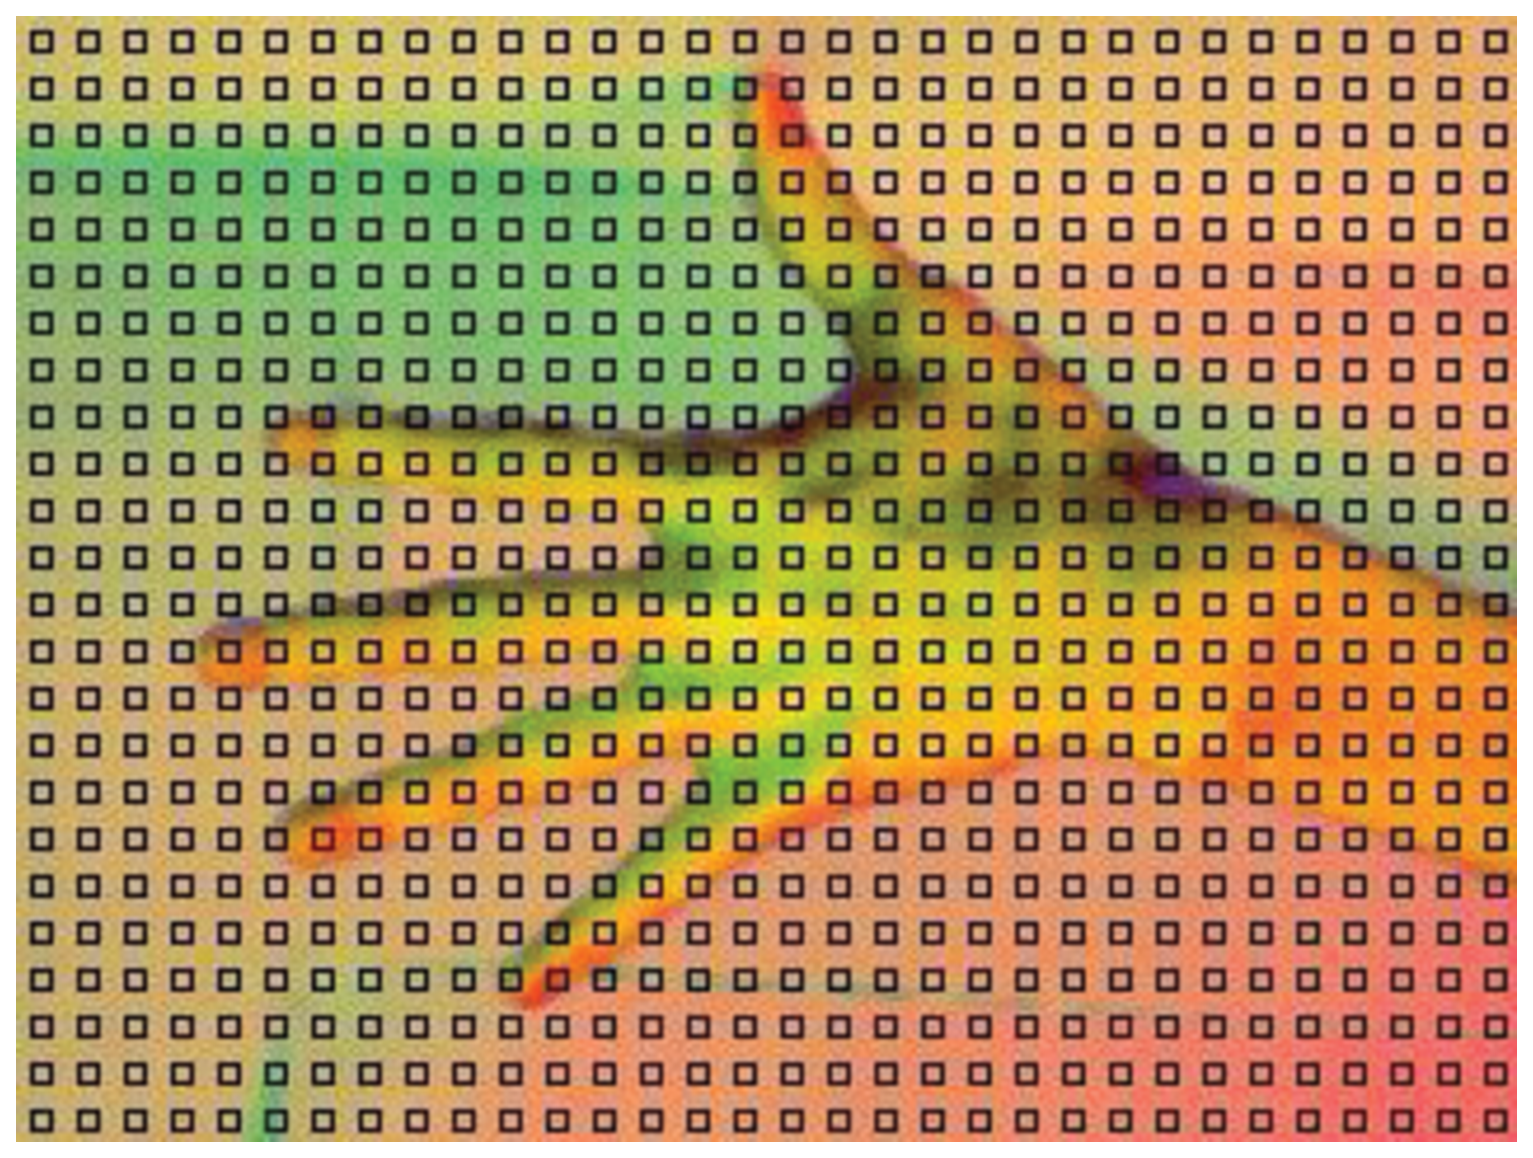
\includegraphics[width=10cm]{Simulator_grid.eps} \\
 \vspace{1mm}
  図4-3. 格子点のイメージ
\end{center}

これらの格子点と重なっている画素について、青色かどうかを判定する。図の4-4は、青色ではない部分を描画したものである。この一連の流れで、レーザー光を用いた際と同じデータを取得することができる。これを横についても、同じことを行う。

\begin{center}
  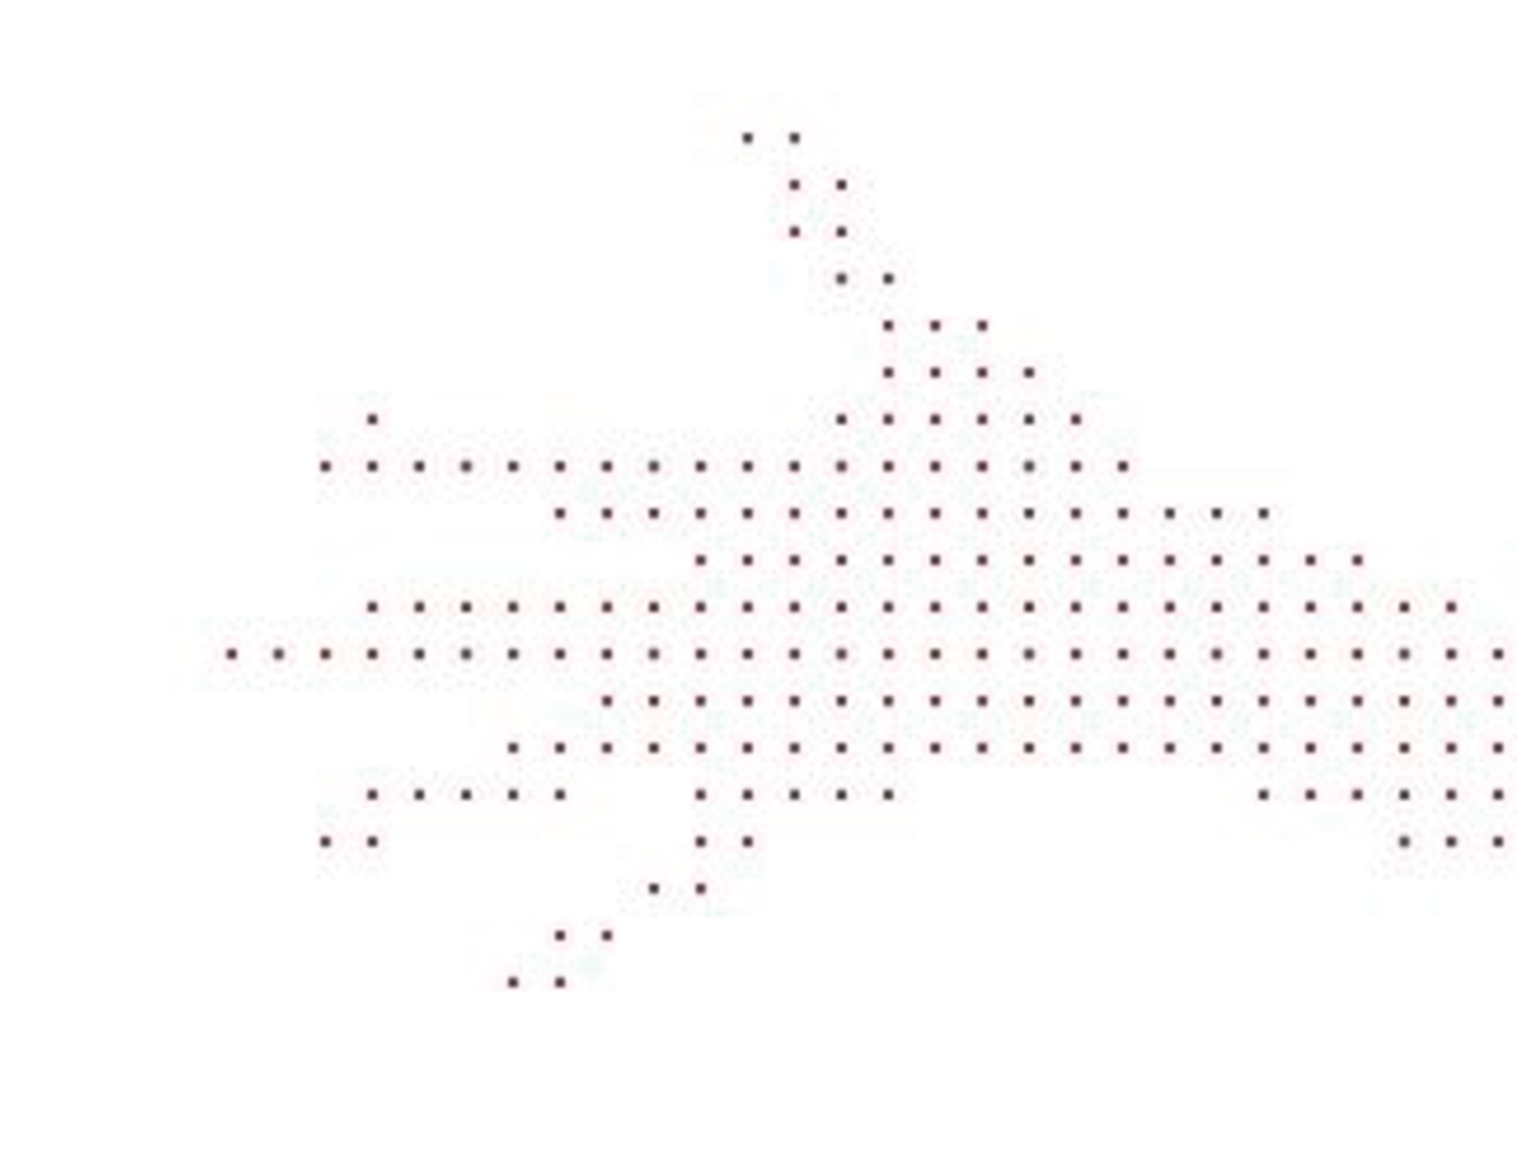
\includegraphics[width=10cm]{Simulator_data.eps} \\
 \vspace{1mm}
  図4-4. 青色ではない部分を描画
\end{center}



\newpage
% 4.2
\subsection{二次元物体データから三次元データを生成}
Webカメラから取得したデータから三次元データを生成する。図4-5、図4-6はそれぞれ縦に設置したカメラ、横に設置したカメラから得たデータとなっている。

 \vspace{5mm}
\begin{minipage}{0.5\hsize}
  \begin{center}
   
\includegraphics[width=70mm]{Simulator_data_h.eps}
   図4-5. 縦に設置したカメラから得たデータ
  \end{center}
  \label{fig:one}
 \end{minipage}
 \begin{minipage}{0.5\hsize}
  \begin{center}
   
\includegraphics[width=70mm]{Simulator_data_v.eps}
   図4-6. 横に設置したカメラから得たデータ
  \end{center}
  \label{fig:two}
 \end{minipage}
 
 始めに、横のカメラから得たデータを元に、Y=0から物体が存在するという情報があるか検索する。存在する情報が発見された時、Xの値を一旦保存する。縦のカメラから得たデータにおいて、先ほど保存したXの値を用いて、物体が存在する情報がないのか検索する。存在する情報が発見された時、Zの値を保存する。この時の、X、Y、Zには物体が存在すると判定する。これをすべてのX、Y、Zについて繰り返し行うことで、三次元のデータを生成する。実際に、図4-5、図4-6から生成した三次元のデータが、図4-7となる。
 
\begin{center}
  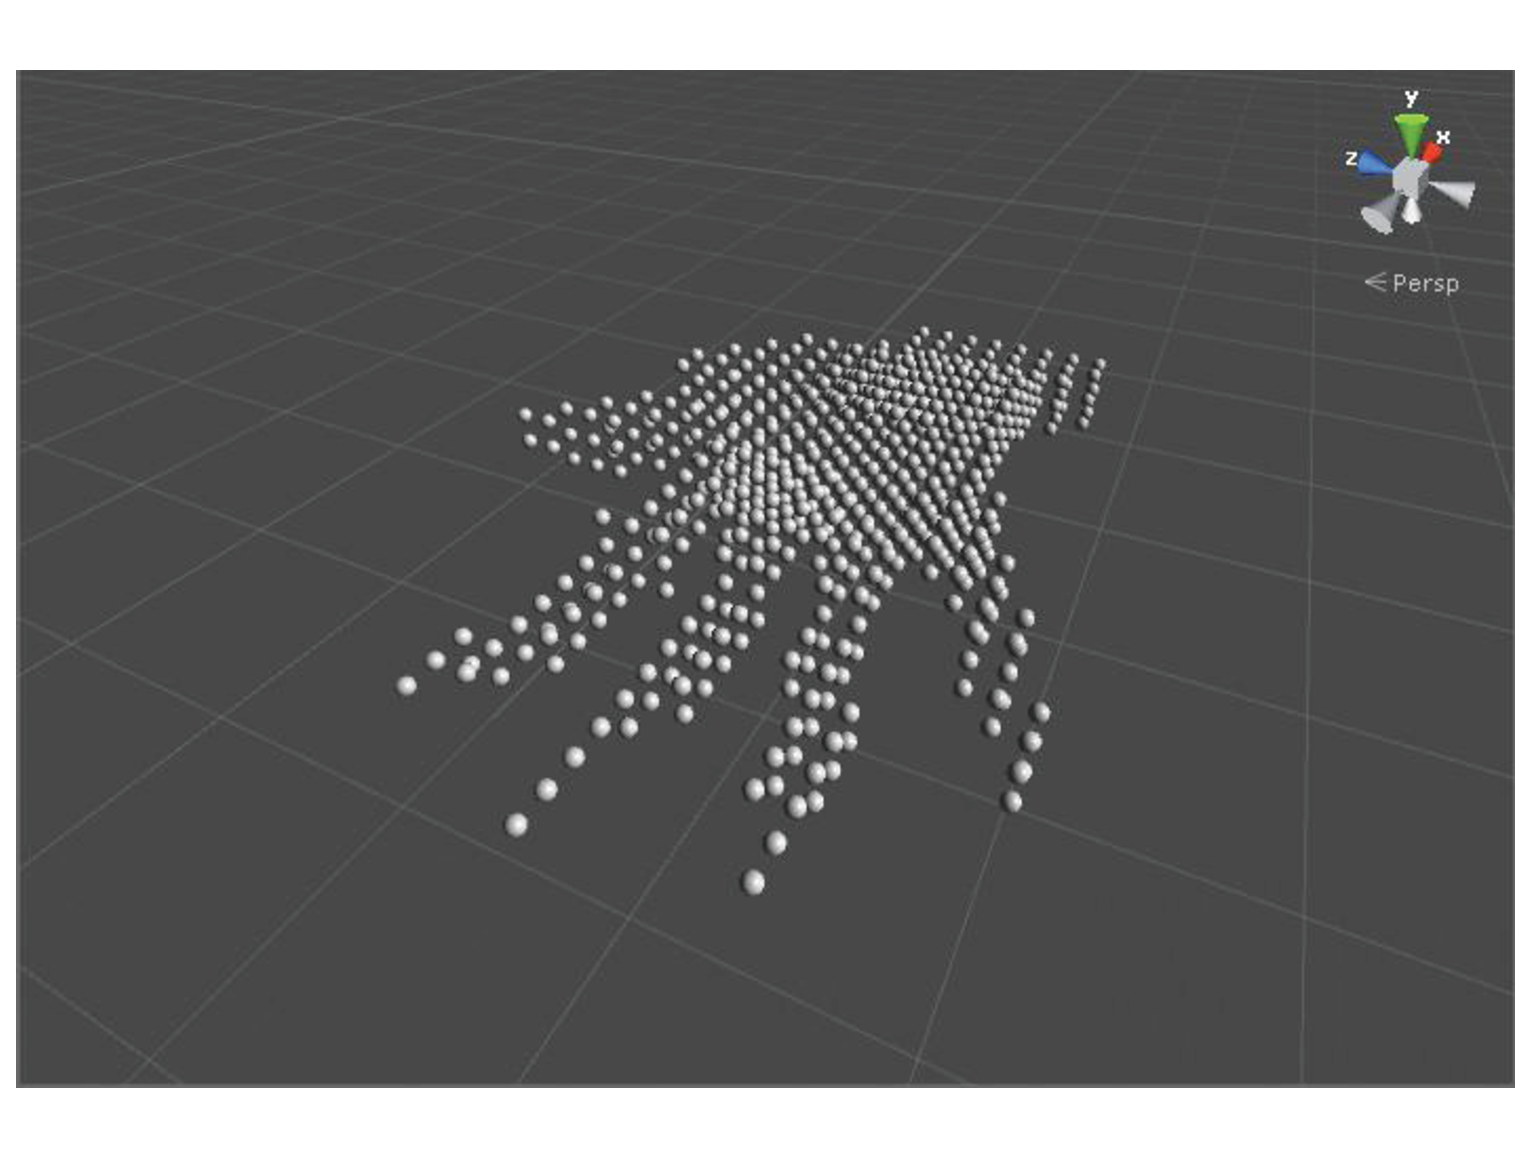
\includegraphics[width=10cm]{Simulator_data_3d.eps} \\
 \vspace{1mm}
  図4-7. 生成した三次元データ
\end{center}



\newpage
% 4.3
\subsection{格子点の内部外部判定}
オブジェクトが存在する三次元空間に、正方格子点が存在すると考える。それらの点がオブジェクトの内部にあるか、外部にあるのかを判定する。三次元空間を一定間隔の層に分けて、各階層毎に内部外部判定を行うことで、擬似的に三次元オブジェクトに対して内部外部判定を行うことができる。各階層毎の内部外部判定には、外積計算と Cauchy の積分定理を組み合わせた手法を用いる。

ここで、外積計算による判定方法と、 Cauchy の積分定理による判定方法について説明を行う。一般的な特徴として、外積計算による方法は、くぼみや穴などを有するドーナッツ型の図形に対する内部外部判定が不利であり、かつ複雑形状の図形において、境界線から離れた内部で判定が困難である。Cauchy の積分定理による方法は、くぼみや穴などを有するドーナッツ型の図形に対する内部外部判定が有利である一方で、複雑形状の図形において、境界線付近での判定に難があるというデメリットが存在する。そこで Cauchy の積分定理の弱点を、外積計算による方法で補うことを考える。しかしながら、外積計算による方法は、複雑形状における内部外部判定で誤判定が引き起こすことが多い。そこで外積計算計算による方法の改良版を使用する。既存の方法では、調査点Pと多角形の輪郭を構成する2点 $z(k),z(k+1)$ の合計三点を用いて計算を行っている。改良版は、調査点Pと輪郭を構成する三点 $z(k-1),z(k),z(k+1)$ の合計四点を用いて計算を行う。

\subsubsection{$z(k-1),z(k),z(k+1)$ の三点が、この順番で左回りに三角形を構成している場合}

\begin{center}
  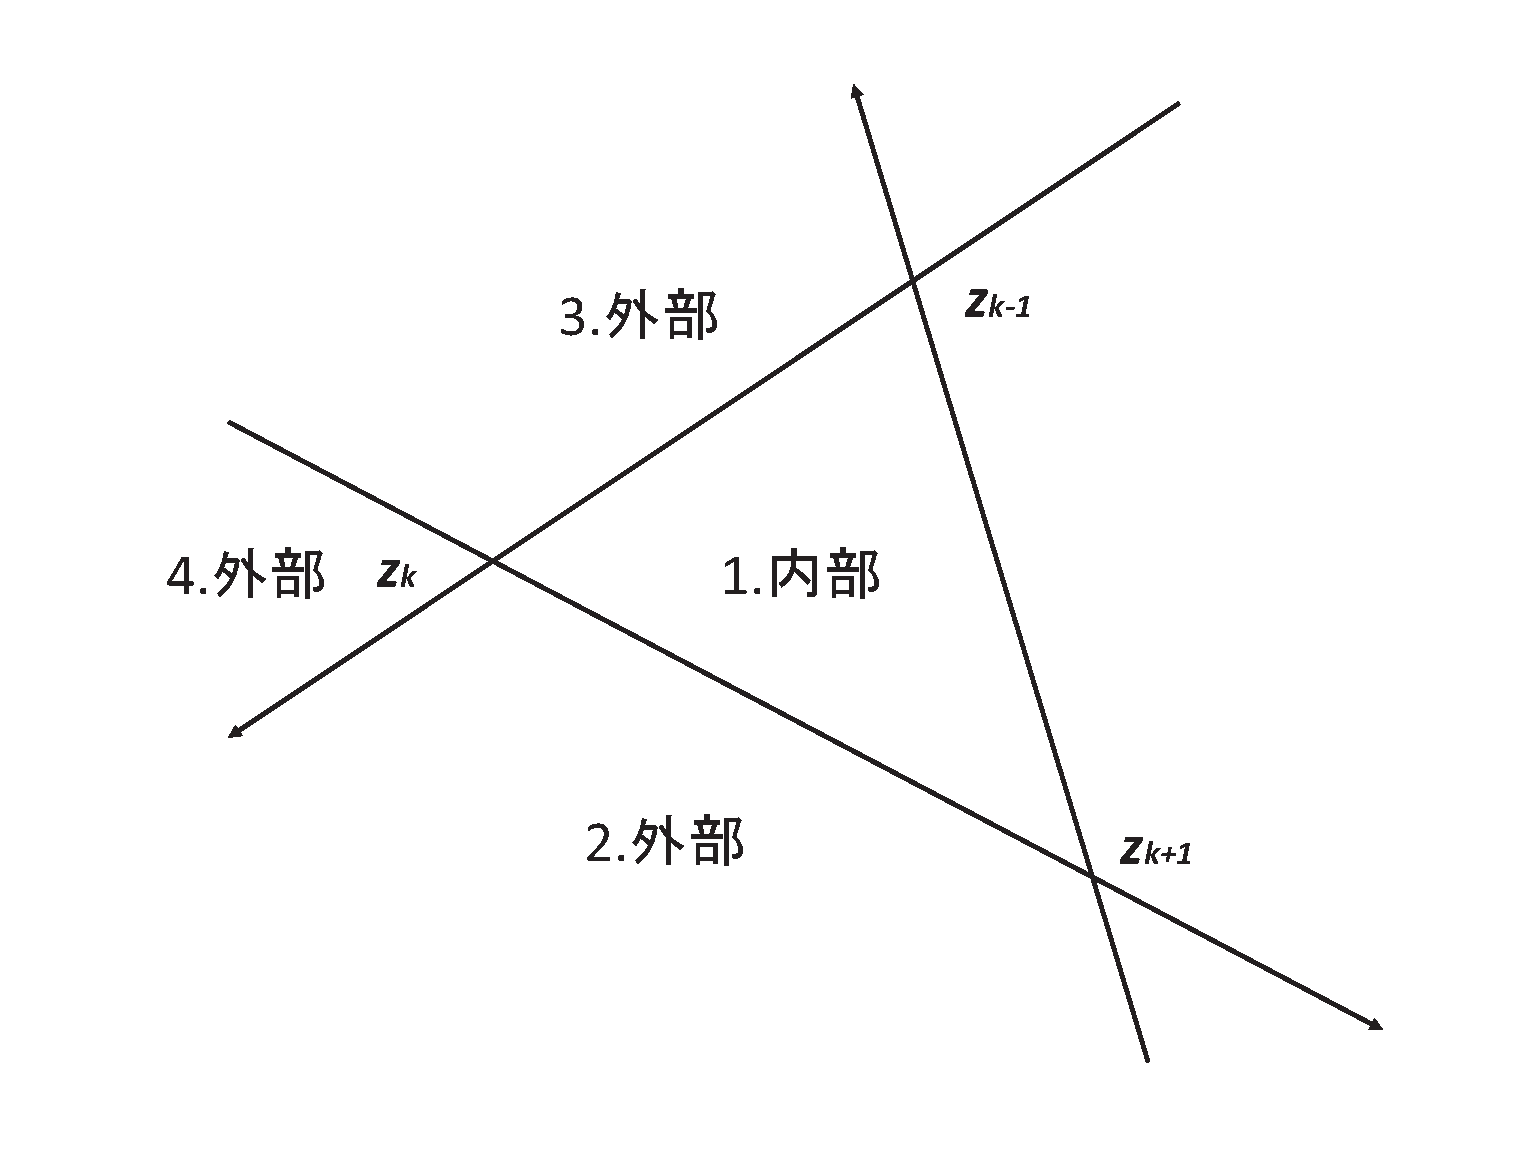
\includegraphics[width=10cm]{hidarimawari_vec.eps} \\
 \vspace{-1mm}
  図4-8. 三点が左回りの三角形
\end{center}

\begin{enumerate}
 \item ベクトル $p z(k-1)$ と ベクトル $z(k-1) z(k)$ の外積の値が0以上、かつベクトル $p z(k)$ とベクトル $z(k) z(k+1)$ の外積の値が0以上ならば内部と判定する。
 \item ベクトル $p z(k-1)$ と ベクトル $z(k-1) z(k)$ の外積の値が0以上、かつベクトル $p z(k)$ とベクトル $z(k) z(k+1)$ の外積の値が負ならば外部と判定する。
 \item ベクトル $p z(k-1)$ と ベクトル $z(k-1) z(k)$ の外積の値が負であり、かつベクトル $p z(k)$ とベクトル $z(k) z(k+1)$ の外積の値が0以上ならば外部と判定する。
 \item ベクトル $p z(k-1)$ と ベクトル $z(k-1) z(k)$ の外積の値が負であり、かつベクトル $p z(k)$ とベクトル $z(k) z(k+1)$ の外積の値が負ならば外部と判定する。
\end{enumerate}

\subsubsection{$z(k-1),z(k),z(k+1)$ の三点が、この順番で右回りに三角形を構成している場合}

\begin{center}
  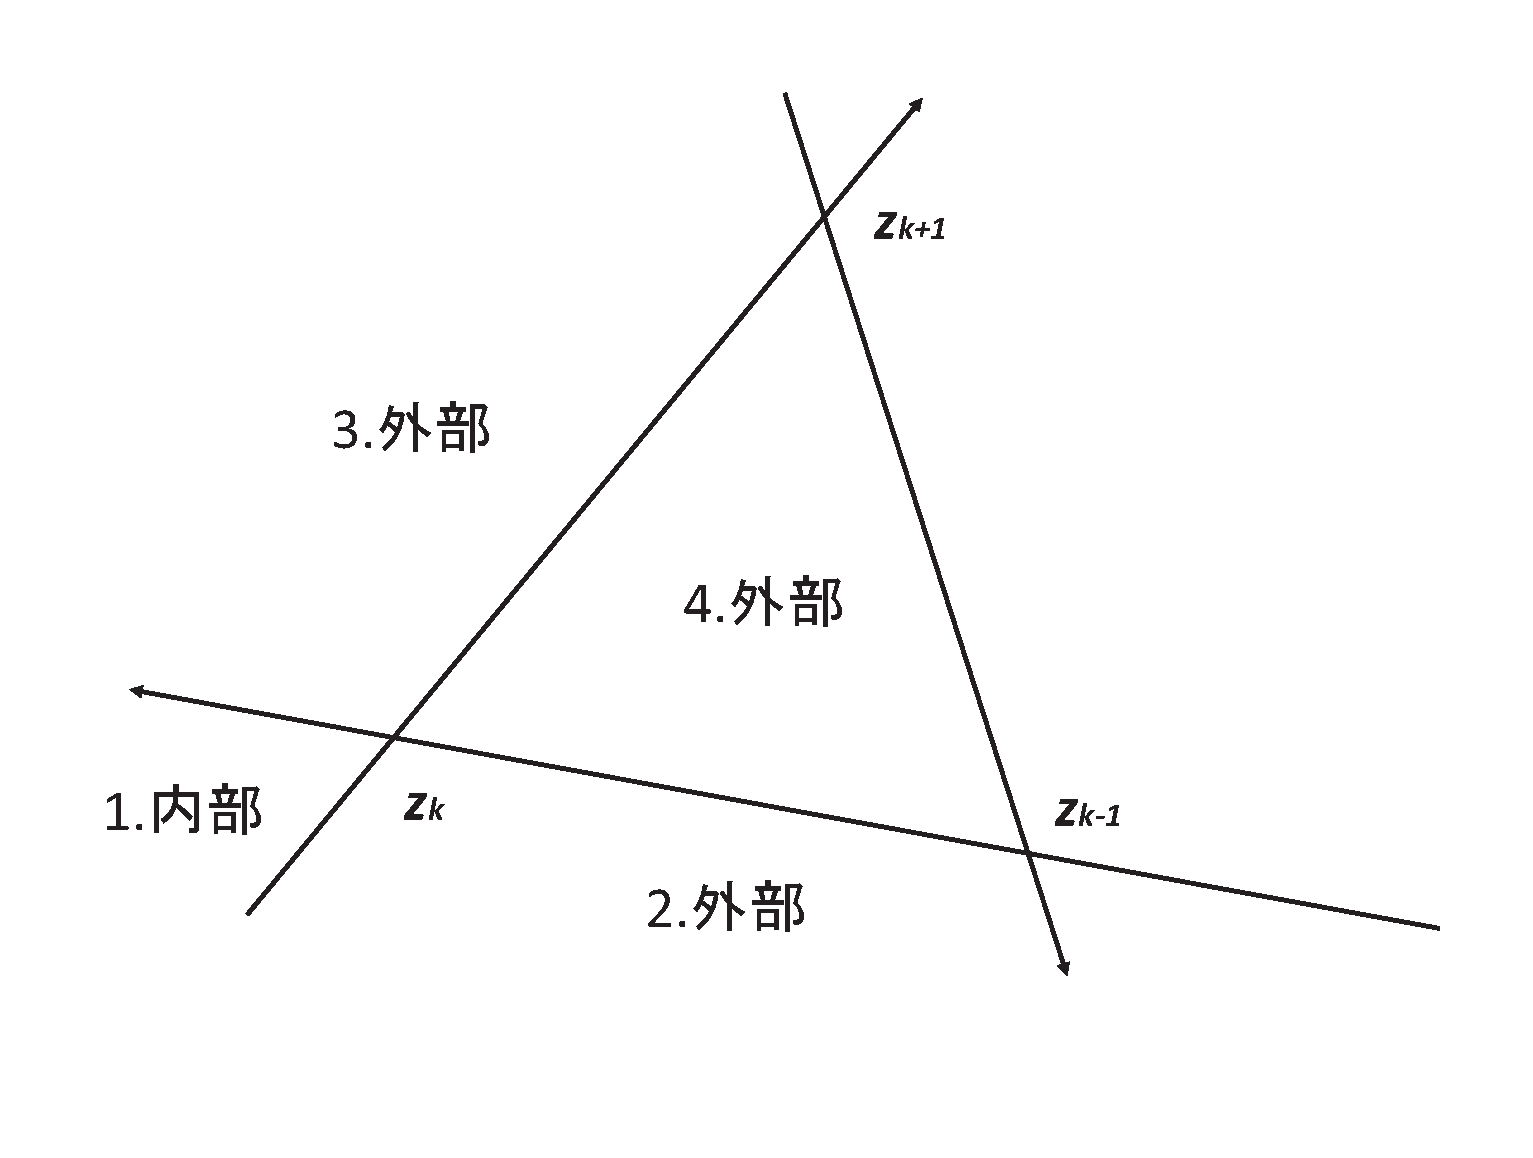
\includegraphics[width=10cm]{migimawari_vec.eps} \\
 \vspace{-1mm}
  図4-9. 三点が右回りの三角形
\end{center}

\begin{enumerate}
 \item ベクトル $p z(k-1)$ と ベクトル $z(k-1) z(k)$ の外積の値が0以上、かつベクトル $p z(k)$ とベクトル $z(k) z(k+1)$ の外積の値が0以上ならば内部と判定する。
 \item ベクトル $p z(k-1)$ と ベクトル $z(k-1) z(k)$ の外積の値が0以上、かつベクトル $p z(k)$ とベクトル $z(k) z(k+1)$ の外積の値が負ならば外部と判定する。
 \item ベクトル $p z(k-1)$ と ベクトル $z(k-1) z(k)$ の外積の値が負であり、かつベクトル $p z(k)$ とベクトル $z(k) z(k+1)$ の外積の値が0以上ならば外部と判定する。
 \item ベクトル $p z(k-1)$ と ベクトル $z(k-1) z(k)$ の外積の値が負であり、かつベクトル $p z(k)$ とベクトル $z(k) z(k+1)$ の外積の値が負ならば外部と判定する。
\end{enumerate}

\subsubsection{$z(k-1),z(k),z(k+1)$ の三点が、この順番で右回りに三角形を構成していない場合}

\begin{center}
  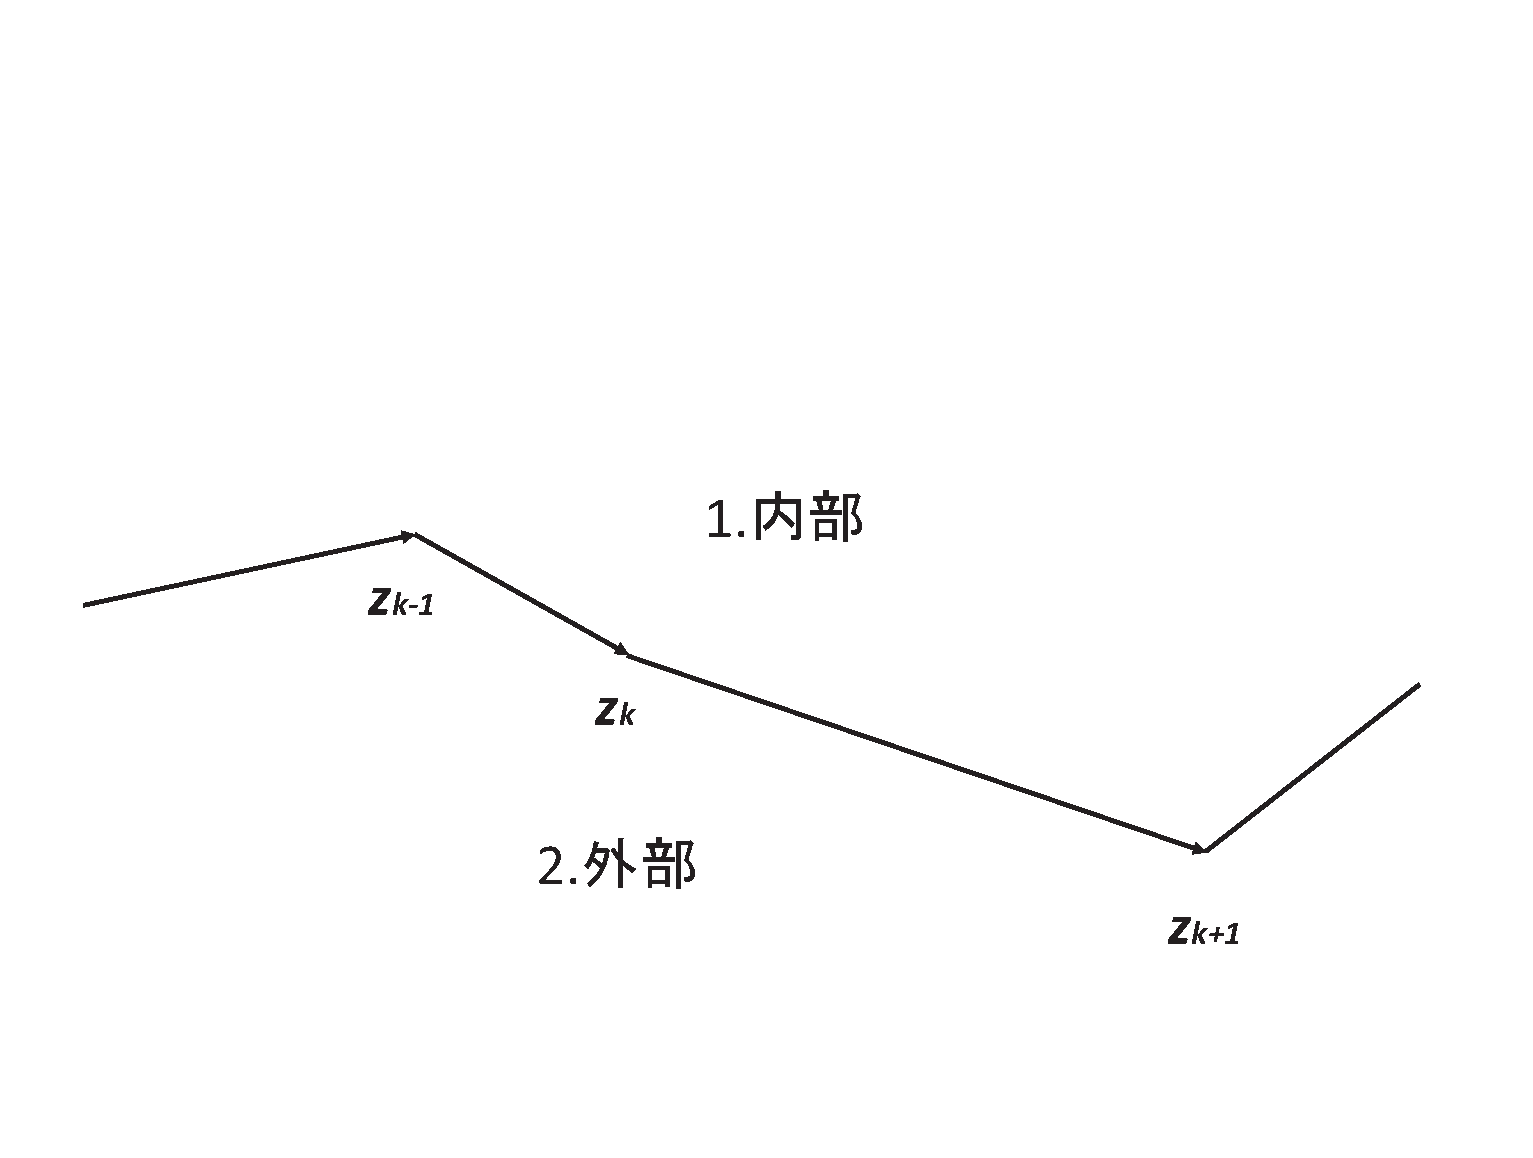
\includegraphics[width=10cm]{sen_vec.eps} \\
 \vspace{-1mm}
  図4-11. 三点が三角形を構成していない
\end{center}

\begin{enumerate}
 \item ベクトル $p z(k)$ と ベクトル $z(k) z(k+1)$ の外積の値が0以上ならば内部と判定する。
 \item ベクトル $p z(k)$ と ベクトル $z(k) z(k+1)$ の外積の値が負ならば外部と判定する。
\end{enumerate}
この場合、ベクトル $p z(k)$ と ベクトル $z(k) z(k+1)$ の外積の値の代わりに、ベクトル $p z(k-1)$ と ベクトル $z(k-1) z(k)$ の外積の値を用いることも可能である

実際にこのアルゴリズムを使用して、内部外部判定を行った結果が図4-11となる。

\vspace{-5mm}
\begin{center}
  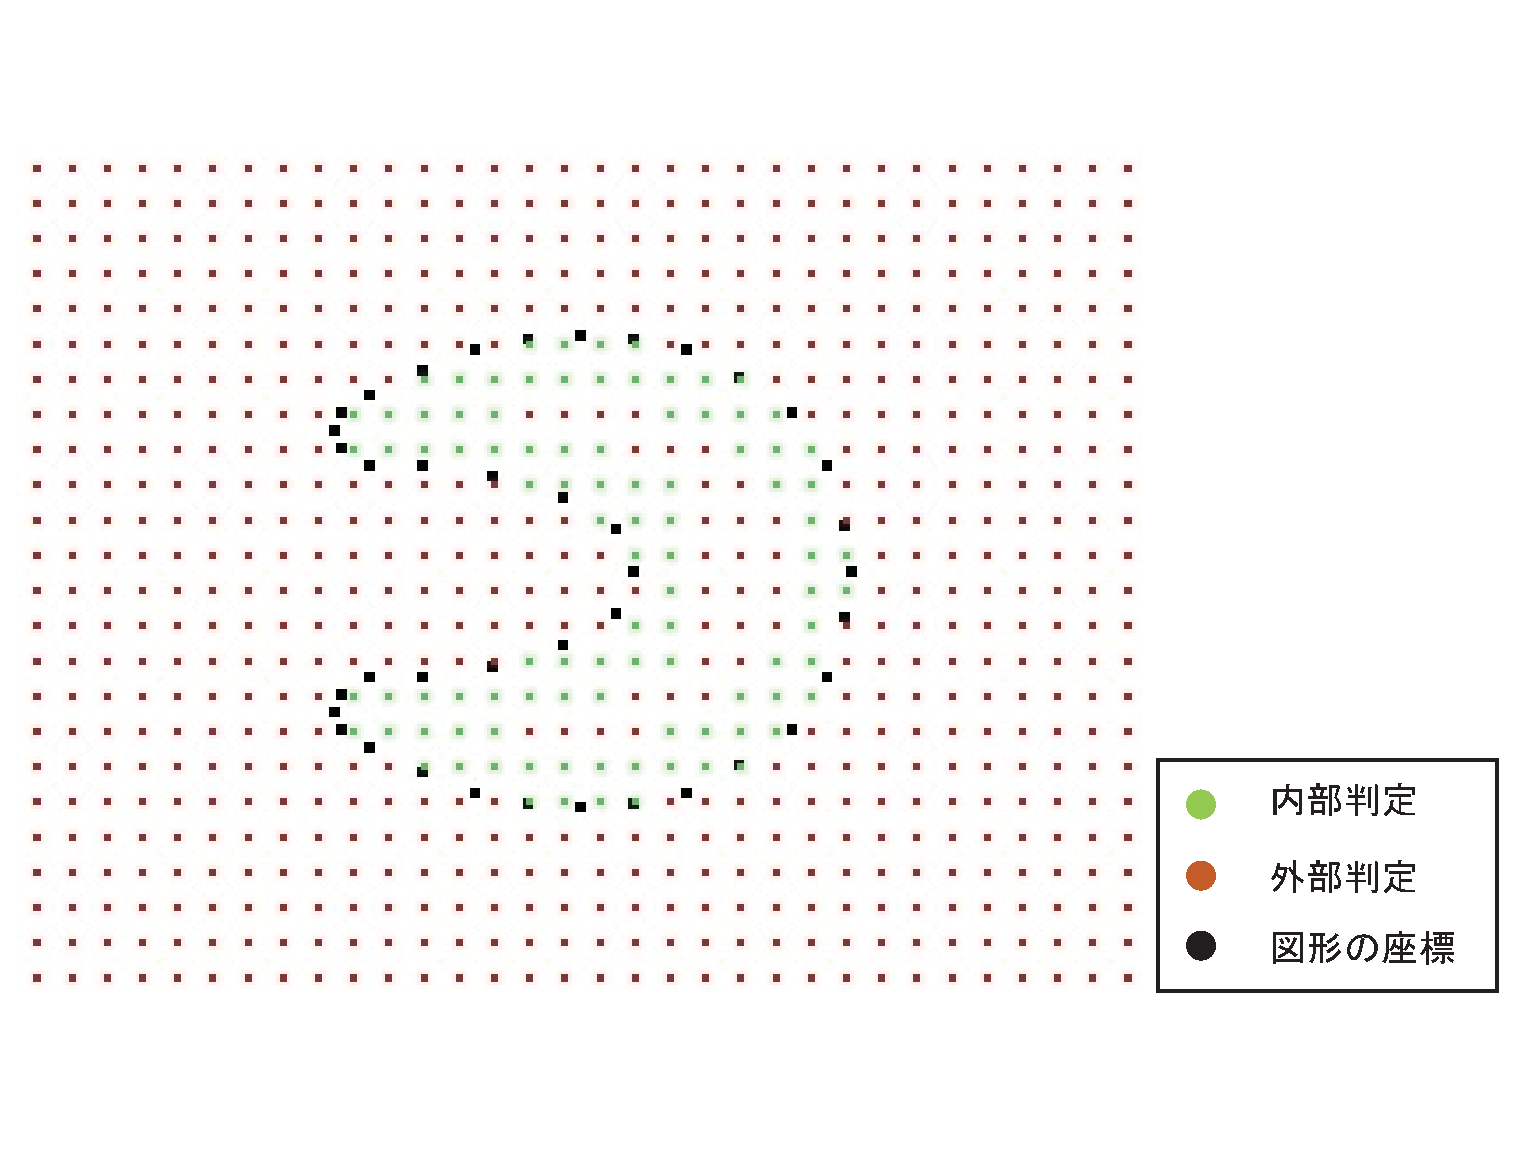
\includegraphics[width=14cm]{Cross_result.eps} \\
 \vspace{-10mm}
  図4-11. 改良版の外積計算による内部外部判定
\end{center}

図を見ると、境界線付近にて正しく判定できていることが分かる。しかしながら、境界線から離れた内部の格子点が正しく判定されていない。

Cauchy の積分定理による方法は、くぼみや穴などを有するドーナッツ型の図形に対する内部外部判定が有利である一方で、複雑形状の図形において、境界線付近での判定に難があるというデメリットが存在する。実際にCauchy の積分定理によって内部外部判定を行った結果が、図5-9となる。

\vspace{-5mm}
\begin{center}
  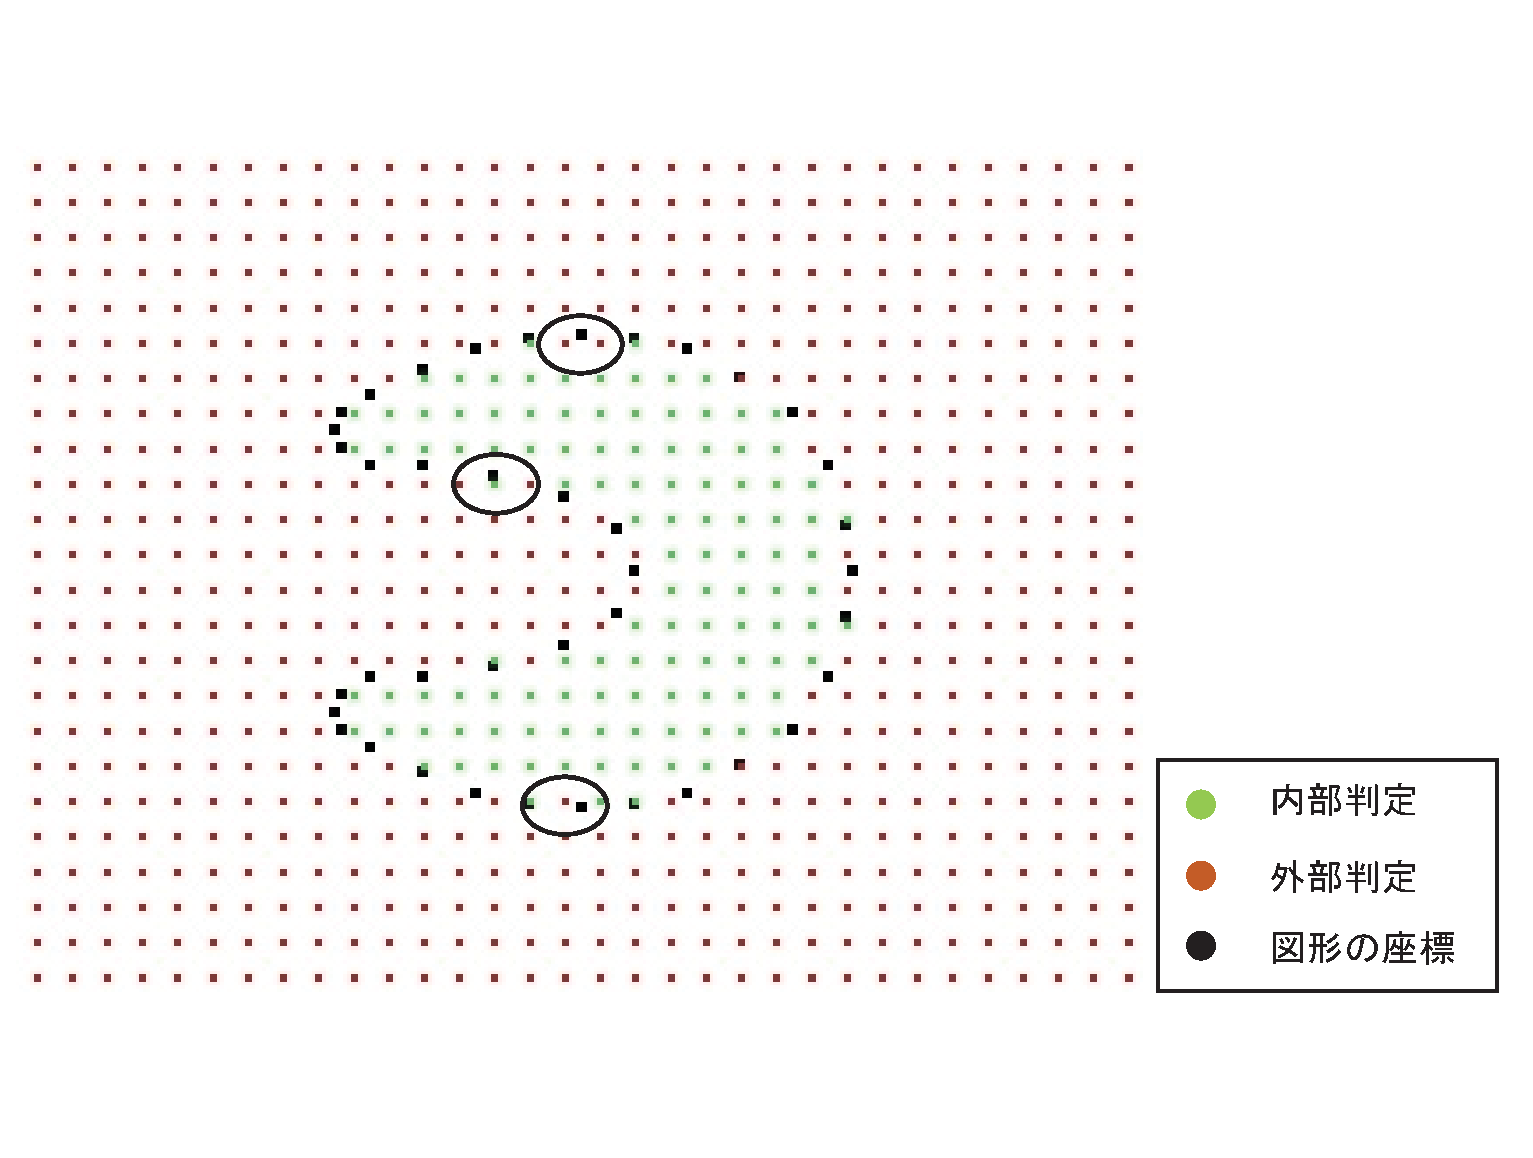
\includegraphics[width=14cm]{Cauchy_result.eps} \\
 \vspace{-10mm}
  図4-12. Cauchyの積分定理による内部外部判定
\end{center}

図を見ると、円で囲まれた格子点が正しく判定されていないことが分かる。

以上の結果を踏まえて、それぞれの方法のデメリットを補うように組み合わせた手法を用いることにする。具体的には、境界線付近の領域では、改良版の外積計算による方法を使用し、境界線から離れた領域では Cauchy の積分定理による方法を使用する。この手法をもとに、内部外部判定を行った結果が、図4-10となる。

\begin{center}
  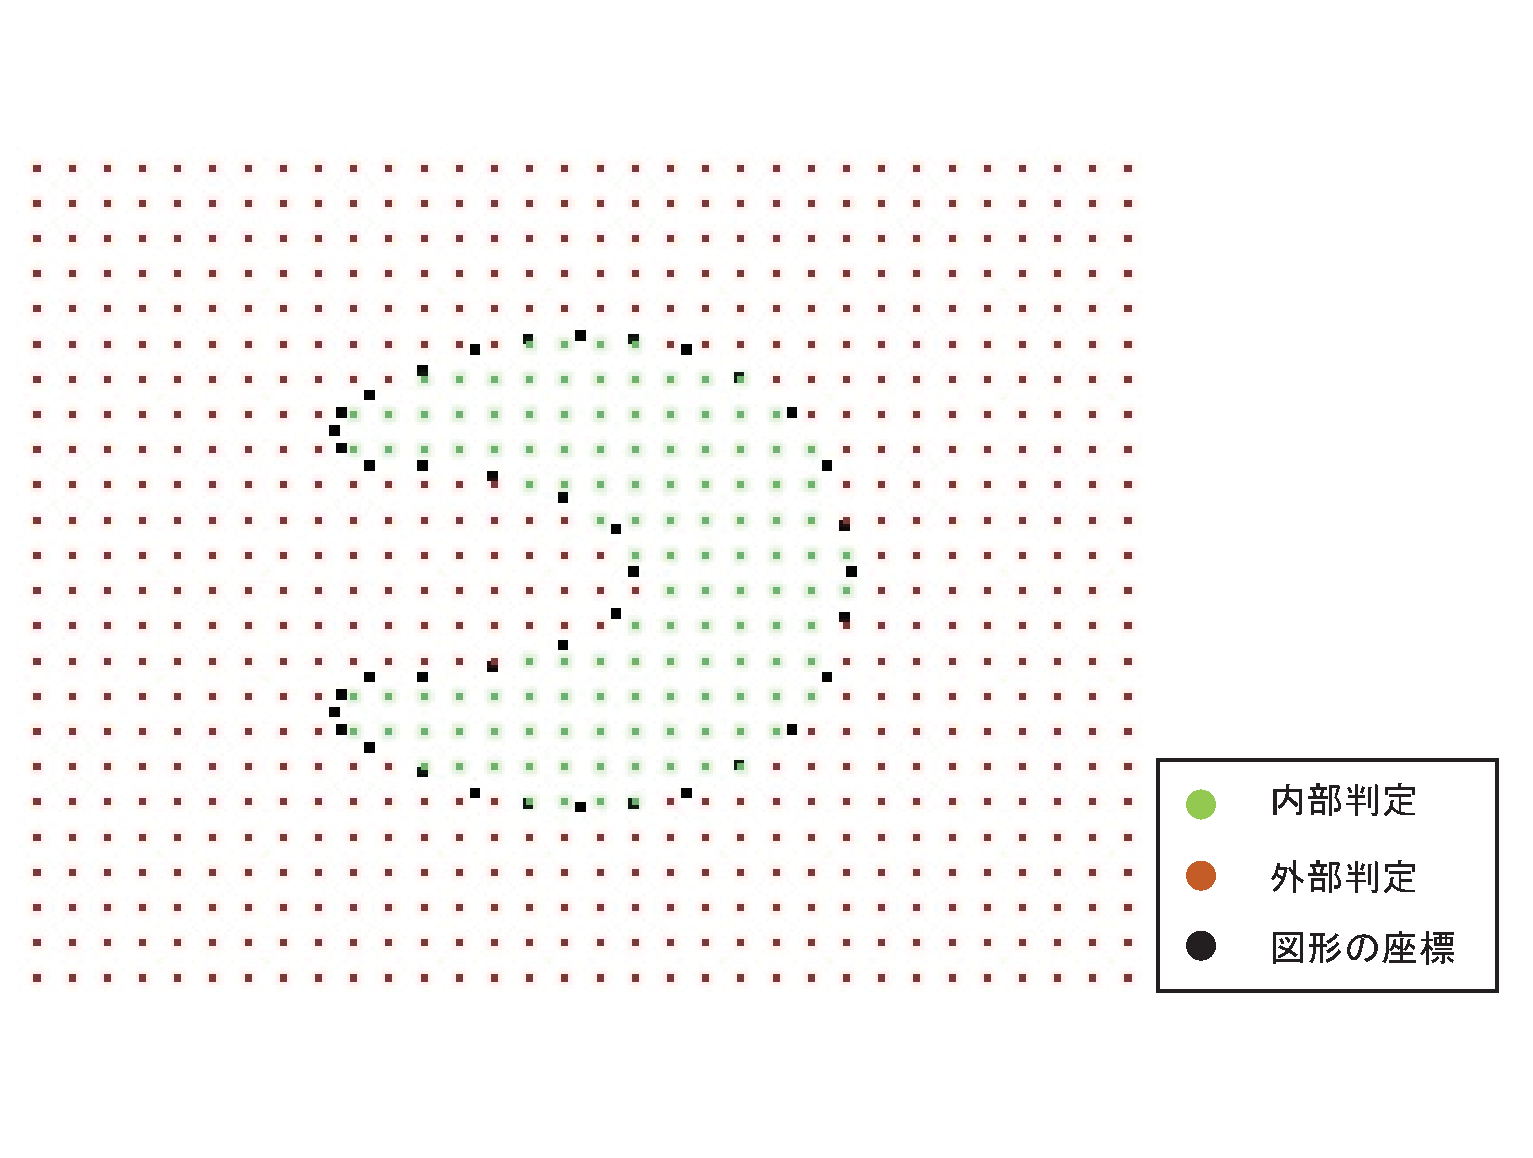
\includegraphics[width=14cm]{Cross-Cauchy_result.eps} \\
 \vspace{-5mm}
  図4-13 外積計算とCauchyの積分定理を組み合わせた判定
\end{center}

改良版の外積計算、および Cauchy の積分定理のそれぞれのデメリットが上手く補われて、すべての格子点について正しく判定されている。同様の処理をすべての階層で行うことで、三次元空間の格子点に対して内部外部判定を行う。


